\documentclass[12pt]{article}
\usepackage[T1]{fontenc}
\usepackage[a4paper, total={7in, 10in}]{geometry}
\usepackage{graphicx}
\usepackage[export]{adjustbox}
\usepackage[font=normalsize,labelfont=bf]{caption}
\usepackage{caption}
\usepackage{subcaption}
\usepackage{float}
\usepackage{titling}
\usepackage{fancyhdr}
\usepackage{lipsum}
\usepackage{amsmath}
\usepackage{siunitx} % For SI unit formatting
\usepackage{booktabs}
\usepackage[polish]{babel}
\newcommand{\mytitle}{WYZNACZANIE CZĘSTOŚCI DRGAŃ WŁASNYCH PRĘTA}
\newcommand{\mysubtitle}{Sprawozdanie}
\fancyfoot{}
\fancyhead[L]{\mytitle}
\fancyhead[R]{\mysubtitle}

\fancyfoot[C]{\thepage}


\renewcommand\maketitlehooka{\null\mbox{}\vfill}
\renewcommand\maketitlehookd{\vfill\null}
\renewcommand{\figurename}{Rysunek}
\renewcommand{\tablename}{Tabela}
\graphicspath{{./tex_resources/}}
\title{\mytitle \\
  \large \mysubtitle}
\author{Mateusz Klisiewicz, Bartek Misiurski, Bartłomiej Szewczak, \\Maksymilian Bąkała, Tomasz Olczak, Aleksander Abramowicz, \\Jakub Waśniewski, Kacper Tukiendorf, Mateusz Brauła, \\Mateusz Gutowski\thanks{Na podstawie \textit{Drgania mechaniczne – Laboratorium; Praca zbiorowa pod redakcją Z. Gałkowski; Oficyna Wydawnicza PW; 1999}}}
\date{\today}
\begin{document}
\pagestyle{fancy}
\maketitle
\newpage
\section*{Wstęp}
Przedmiotem badania były dwa pręty, jeden wykonany z włókna szklanego a drugi z brązu. Pręty utwierdzono w aparaturze (Rys. 1) i poddawano działaniu okresowej siły. w celu określenia ich częstości drgań własnych. 
\begin{figure}[H]
		\centering
		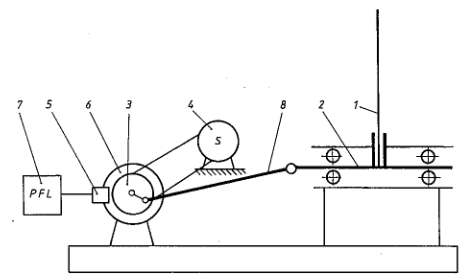
\includegraphics[width=10cm]{sch}
		\caption{Schemat stanowiska pomiarowego}
		\label{rys:comb1}
\end{figure}
\section*{Wyniki Pomiarów}
Właściwości fizyczne obydwu prętów zmierzono i umieszczono w Tabeli 1.
\begin{table}[h!]
\centering
\begin{tabular}{lcc}
\toprule
Właściwość & Pręt z Brązu & Pręt z Włókna Szklanego\\
\midrule
Moduł Younga, $E$ & \SIrange{100}{120}{\giga\pascal} & \SI{69.5}{\giga\pascal} \\
Średnica, $d$ & \SI{0,009}{\meter} $\pm$ \SI{0,001}{\meter} & \SI{0.01}{\meter} $\pm$ \SI{0,001}{\meter} \\
Geometryczny Moment Bezwładności, $J$ & \(\frac{\pi d^4}{64}\) & \(\frac{\pi d^4}{64}\) \\
Długość, $l$ & \SI{2.89}{\meter} $\pm$ \SI{0,001}{\meter} & \SI{2.6}{\meter} $\pm$ \SI{0,001}{\meter} \\
Masa, $m$ & \SI{1.55}{\kilogram} $\pm$ \SI{0,01}{\kilogram} & \SI{0.39}{\kilogram} $\pm$ \SI{0,01}{\kilogram} \\
\bottomrule
\end{tabular}
\caption{Właściwości fizyczne badanych prętów.}
\label{table:properties}
\end{table}
\\Za pomocą pokrętła zwiększano częstotliwość siły wymuszającej. aż do zaobserwowania rezonansu drgań układu. W ten sposób ustalono częstotliwości rezonansowe prętów dla trzech postaci drgań (Tab. 2).
\begin{table}[h!]
\centering
\resizebox{\textwidth}{!}{%
\begin{tabular}{lcccccc}
\toprule
Postać Drgań & \multicolumn{2}{c}{$n=1$} & \multicolumn{2}{c}{$n=2$} & \multicolumn{2}{c}{$n=3$} \\
 & [\si{\hertz}] &[ \si{\radian\per\second}] & [\si{\hertz}] & [\si{\radian\per\second}] & [\si{\hertz}] & [\si{\radian\per\second}] \\
\midrule
Pręt z Brązu & $1,083 \pm 0,017$ & $2,167\pi \pm 0,033 \pi $ & $3,050 \pm 0,017$ & $6,1\pi \pm 0,033 \pi  $ & $4,883 \pm 0,017 $ & $9,767\pi \pm 0,033 \pi $ \\
Pręt z Włókna Szklanego & $2 \pm 0,017 $& $4\pi \pm 0,033 \pi $ & $5,833 \pm 0,017 $ & $11,667\pi \pm 0,033 \pi $ & $13,833 \pm 0,017 $ & $27,667\pi \pm 0,033 \pi  $ \\
\bottomrule
\end{tabular}%
}
\caption{Zmierzone wartości częstotliwości rezonansowych badanych prętów.}
\label{table:frequencies}
\end{table}
\newpage
Na podstawie zależności wyprowadzonych w instrukcji do ćwiczenia:\\

\begin{gather}
(\kappa l)_n=\frac{2n-1}{2}\pi \\
\omega=\kappa^2\sqrt{\frac{l}{m} EJ} 
\end{gather}
Rugując $\kappa$:
\begin{equation}
\omega_n=\frac{\pi \sqrt{\frac{l}{m} E J }}{4 l^{2}} (2 n - 1)^{2}
\end{equation}\\
Otrzymano zależność częstości własnej $\omega_{n}$ od postaci drgań $n$ $(3)$. Obliczono wartości teoretyczne $\omega_t$ i zestawiono je w tabeli razem z wartościami eksperymentalnymi $\omega_e$(Tab. 3).

\begin{table}[h!]
\centering
\begin{tabular}{lcccc}
\toprule
 & \multicolumn{2}{c}{Pręt z Brązu} & \multicolumn{2}{c}{Pręt z Włókna Szklanego} \\
\cmidrule(lr){2-3} \cmidrule(lr){4-5}
$n$ & \(\omega_{\text{e}} \, (\si{\radian\per\second})\) & \(\omega_{\text{t}} \, (\si{\radian\per\second})\)  & \(\omega_{\text{e}} \, (\si{\radian\per\second})\) & \(\omega_{\text{t}} \, (\si{\radian\per\second})\)  \\
\midrule
1 & \(2,167\pi  \pm 0,033 \pi\) & \(0,83\pi\) & \(4\pi  \pm 0,033 \pi\) & \(5.505\pi\)  \\
2 & \(6,1\pi  \pm 0,033 \pi\) & \(7,478\pi\) & \(11.667\pi  \pm 0,033 \pi\) & \(49,541\pi\)  \\
3 & \(9,767\pi  \pm 0,033 \pi\) & \(20,771\pi\) & \(27,667\pi  \pm 0,033 \pi\) & \(137,615\pi\) \\
\bottomrule
\end{tabular}
\caption{Porównanie wartości eksperymentalnych i teoretycznych częstości własnych dla badanych prętów.}
\label{table:omega}
\end{table}

\begin{figure}[H]
		\centering
		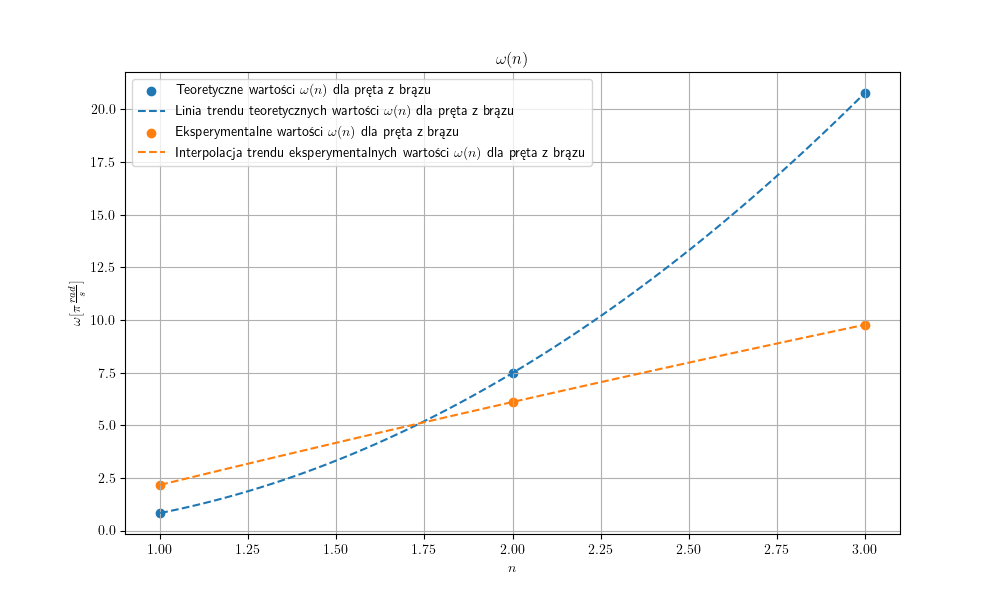
\includegraphics[width=20cm, center]{b1}
		\caption{Zależności teoretyczne i eksperymentalne częstości własnej $\omega$ od postaci drgań $n$dla pręta z brązu}
		\label{rys:b1}
\end{figure}
\section*{Wnioski}
Zmierzone wartości w sposób istotny odbiegają od przewidywanych. Tak znaczna rozbieżność musi wynikać z błędnego przeprowadzenia eksperymentu, lub z wad aparatury pomiarowej. Aby móc wnioskować na temat wyników, konieczne jest ponowne przeprowadzenie badania, po uprzedniej inspekcji stanowiska.
\end{document}